\begin{figure}
\centering
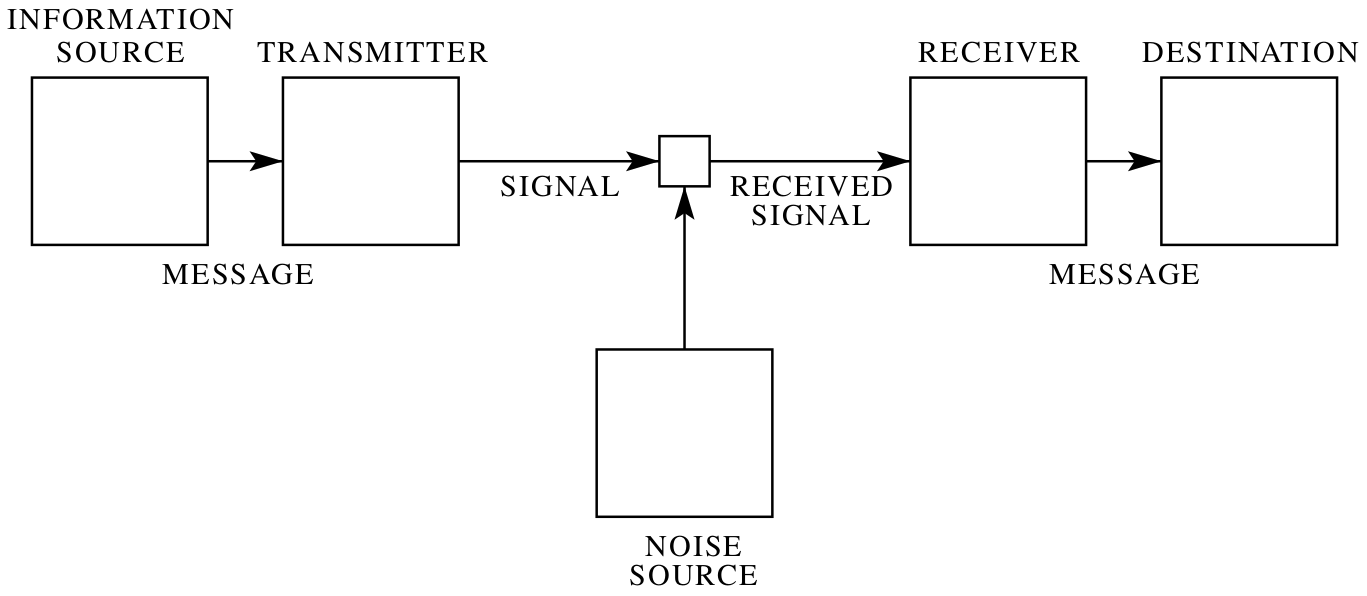
\includegraphics[scale=0.25]{plots/shannon-comm-system.png}
\caption[\label{fig:shannon-comm-system}Shannon's general communication system consists of
an \textit{information source} which produces a message,
a \textit{transmitter} which manipulates the message to produce a signal suitable for transmission over the channel,
a \textit{channel} which serves as the medium for signal transmission from the transmitter to the receiver,
a \textit{receiver} which reconstructs the message from the signal and
a \textit{destination} which is the message's intended point of delivery.]{\label{fig:shannon-comm-system}Shannon's general communication system consists of
an \textit{information source} which produces a message,
a \textit{transmitter} which manipulates the message to produce a signal suitable for transmission over the channel,
a \textit{channel} which serves as the medium for signal transmission from the transmitter to the receiver,
a \textit{receiver} which reconstructs the message from the signal and
a \textit{destination} which is the message's intended point of delivery\protect\footnotemark[1].}
\end{figure}
